\documentclass[convert={density=1200}]{standalone}
\usepackage{tikz}
\usetikzlibrary{shapes.geometric, arrows}
\usetikzlibrary{matrix}
\usetikzlibrary{positioning}

\tikzstyle{server} = [rectangle, rounded corners, text centered, draw=black, fill=green!30, inner sep=5pt]
\tikzstyle{node} = [rectangle, rounded corners, text centered, draw=black, fill=blue!30, inner sep=5pt]
\tikzstyle{action} = [rectangle, text centered, draw=black, inner sep=5pt]
\tikzstyle{trait} = [trapezium, text centered, draw=black, fill=yellow!30, inner sep=5pt, text=red!50!black, font=\ttfamily]

\tikzstyle{server_message} = [thick, green!50!black, dashed,->, >=stealth]
\tikzstyle{node_message} = [thick, blue, dashed, ->, >=stealth]
\tikzstyle{action_step} = [thick, black, ->, >=stealth]

\begin{document}

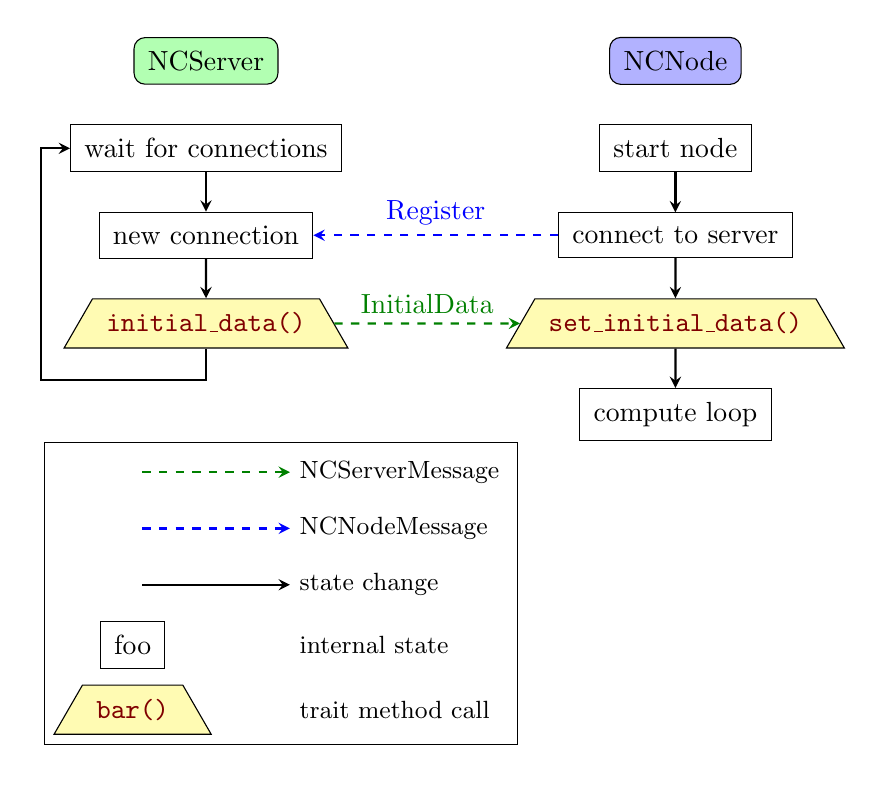
\begin{tikzpicture}

    \matrix [column sep = 20mm, row sep = 5mm] {
        \node (ncserver) [server] {NCServer}; &
        \node (ncnode) [node] {NCNode}; \\

        \node (wait) [action] {wait for connections}; &
        \node (start) [action] {start node}; \\

        \node (connected) [action] {new connection}; &
        \node (connect) [action] {connect to server}; \\

        \node (initial) [trait] {initial\_data()}; &
        \node (set_initial) [trait] {set\_initial\_data()}; \\

        & \node (loop) [action] {compute loop}; \\
    };

    \draw [action_step] (wait) -- (connected);
    \draw [action_step] (connected) -- (initial);

    \draw [action_step] (start) -- (connect);
    \draw [action_step] (connect) -- (set_initial);
    \draw [action_step] (set_initial) -- (loop);

    \draw [node_message] (connect) -- node [above] {Register} (connected);
    \draw [server_message] (initial) -- node [above] {InitialData} (set_initial);

    % \draw [action_step] (initial) -- node {} ++(0, -0.75) -- node {} ++(-2, 0) -- node {} ++(0, 3) -- (wait);
    \draw [action_step] (initial.south) |- ++(-2.1, -0.4) |- (wait.west);


    % Add bottom page border with invisible node
    \node at (0, -6.5) {};

    % Add left page border with invisible node
    \node at (-5.3, 0) {};

    \matrix [column sep=10mm, row sep=2.0mm, rectangle, draw=black,
             column 2/.style={anchor=west}
        ] at (-2.2, -4.5) {
        \node (label1a) {}; & \node [font=\small] (label1b) {NCServerMessage}; \\
        \node (label2a) {}; & \node [font=\small] (label2b) {NCNodeMessage}; \\
        \node (label3a) {}; & \node [font=\small] (label3b) {state change}; \\
        \node [action] {foo}; & \node [font=\small] {internal state}; \\
        \node [trait] {bar()}; & \node [font=\small] {trait method call}; \\
    };

    \draw [server_message] (label1a) -- (label1b);
    \draw [node_message] (label2a) -- (label2b);
    \draw [action_step] (label3a) -- (label3b);

\end{tikzpicture}

\end{document}
